\section{Complexitat d'Un Algorisme (Big O Notation)}

Abans de veure els alguns dels algorismes aplicats a la programació que existeixen hem d'entendre bé el que és Big O Notation.
Quan parlem de rendiment i optimització, és important tenir una regla per determinar que tan bo o que tan dolent és un algorisme, per això existeix Big O Notation que ens descriu el pitjor escenari, és a dir, el màxim en la quantitat més gran de repeticions que l'algorisme ha d'executar. \newline

Big O Notation és utilitzat a les ciències computacionals per descriure la complexitat i el rendiment d'un algorisme, un factor que hem de tenir en compte és que la majoria d'algorismes canvien el seu rendiment depenent de la quantitat d'input que ha de processar, és a dir alguns algorismes funcionen amb un bon rendiment quan la quantitat de l'input és petit, però perden efectivitat quan incrementes l'input.
Generalment, Big O Notation descriu el pitjor escenari possible, és a dir, el màxim nombre de repeticions que l'algorisme ha d'executar. \newline \newline

\begin{description}

\item[$O(1)$]
\index{algorisme de temps constant}

Aquesta expressió indica temps constant, el que significa és que l'algorisme s'executarà amb el mateix rendiment sense importar la mida de l'input, és a dir, no es veurà afectat per la quantitat de dades que estiguem manejant.
Aquesta notació és la més eficient, òptima i amb el millor rendiment. \newline

\underline{Exemple:} \newline

\begin{lstlisting}
int a = 5;
int b = 10;
int c = a + b;
cout << c << endl; // 15
\end{lstlisting}

\newpage

\item[$O(\log n)$]
\index{algorisme logarítmic}
Aquesta expressió índica que el temps augmenta linealment, mentre que $n$ augmenta exponencialment, per tant, si es triga 1 segon a processar 10 elements, en conseqüència es trigaran 2 segons per calcular-ne 100, 3 per 1000 i així successivament. \newline

\underline{Exemple:} \newline

\begin{lstlisting}
int n;
cin >> n; // Input -> 512

while (n > 1){
    cout << n << " ";
    n = n / 2;
}

// Output -> 512 256 128 64 32 16 8 4 2
\end{lstlisting}

En aquest cas, n = 512, però el programa només es repeteix $\log_{2}(512)$ vegades, és a dir, 9 vegades, ja que a cada pas, dividim $\frac{n}{2}$ . \newline

\item[$O(n)$]
\index{algorisme lineal}

Aquesta expressió indica un creixement lineal, la complexitat de l'algoritme augmenta de manera proporcional a la dimensió de l'input.
Aquesta notació és bastant eficient, i té un molt bon rendiment. \newline

\underline{Exemple:} \newline

\begin{lstlisting}
int n;
cin >> n; // Input -> 8 (per exemple)

for (int i = 1; i <= n; i++){
    cout << i << " " << endl;
}

// Output -> 1 2 3 4 5 6 7 8

\end{lstlisting}

En aquest exemple, el nostre programa ens escriu tots els nombres d'1 fins $n$ i, per tant, s'ha de repetir $n$ vegades. \newpage

\item[$O(n \log n)$]

Aquesta expressió és una fusió de $O(n)$ i de $O(\log n)$.
Es diu que un algorisme té una complexitat temporal quasi lineal $O(n \log n)$ quan cada operació de les dades d'entrada té una complexitat temporal de $O(\log n)$ o quan l'algorisme ordena tota l'entrada i, per tant, és $O(n \log n)$, ja que és el cost de qualsevol algorisme d'ordenació eficient (merge sort, etc.) \newline

\underline{Exemple:} \newline

\begin{lstlisting}
int n;
cin >> n; // Input -> 4

vector llista;
for (int i = n; i >= 1; i--){
    llista.push_back(i);
}

// llista [4, 3, 2, 1]
sort(llista.begin(), llista.end());
// llista [1, 2, 3, 4]

\end{lstlisting}

\item[$O(n^2)$]
\index{algorisme quadràtic}

Aquesta expressió indica que el creixement en complexitat és directament proporcional al quadrat de la mida de l'input.
Aquest algoritme és poc eficient quan l'input és gran i, per tant, és molt poc recomanable. \newline

\underline{Exemple:} \newline

\begin{lstlisting}
int n;
cin >> n; // Input -> 3

for (int i=1; i<=n; i++){
    for (int j=1; j<=n; j++){
        cout << i << " " << j << " ";
    }
}

// Output -> 1 1  1 2  1 3  2 1  2 2  2 3  3 1  3 2  3 3
\end{lstlisting}
\newpage

Cal dir que la complexitat temporal és tan sols una aproximació, per exemple, si un algorisme treballa específicament en temps $O(n + n^2)$, direm simplement que funciona en $O(n^2)$, ja que la suma de $n$ és irrellevant amb el $n^2$ . \newline

\end{description}

\begin{center}
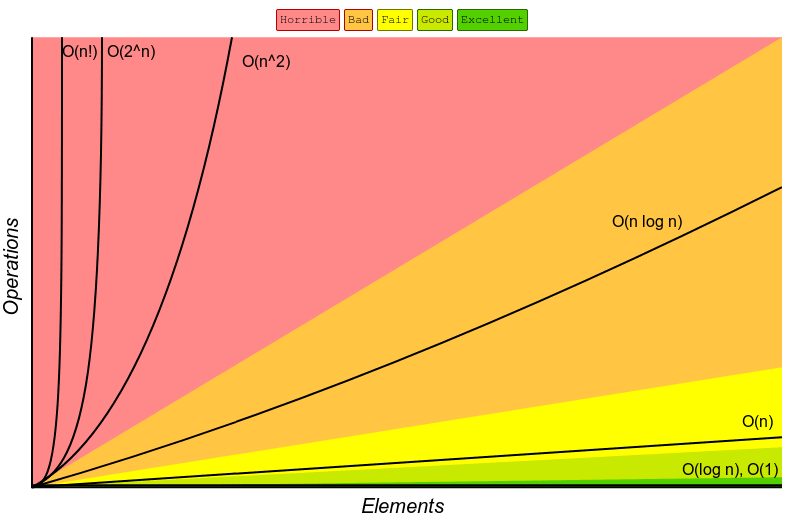
\includegraphics[width=.9\textwidth]{compl.png}

\caption{\emph{Figura 1: Operacions-Temps. Font: \url{https://towardsdatascience.com/understanding-time-complexity-with-python-examples-2bda6e8158a7}}}
\end{center}

A la Figura 1 podem observar la relació Temps-Operacions de les complexitats de $n$ més típiques en la programació, bàsicament el gràfic ens indica el rendiment i l'eficiència de cada complexitat. \newline


